\section{Context}
\label{section:context}

This project is framed within the broad field of \textit{data mining}, emphasizing its relation with \textit{data privacy}. We will provide now definitions and concepts of the main topics of the project’s environment.

\subsection{Data mining}

Today’s information society produces vast amounts of data all over the world. This data comes from innumerable sources and in diverse formats, and has been stored for years in data warehouses, waiting to be processed. With the continuous increase in computing power, due to the recent advances in software and hardware technologies, the machine learning field, more commonly known as \textit{data mining}, has arisen, allowing us to exploit this stored data and distill knowledge from it.

Data mining is, indeed, a holistic process, where many different disciplines are involved, from data acquisition and storage, through its selection, filtering and analysis up to information extraction, visualization and knowledge discovery.

\begin{figure}[h]
	\centering
	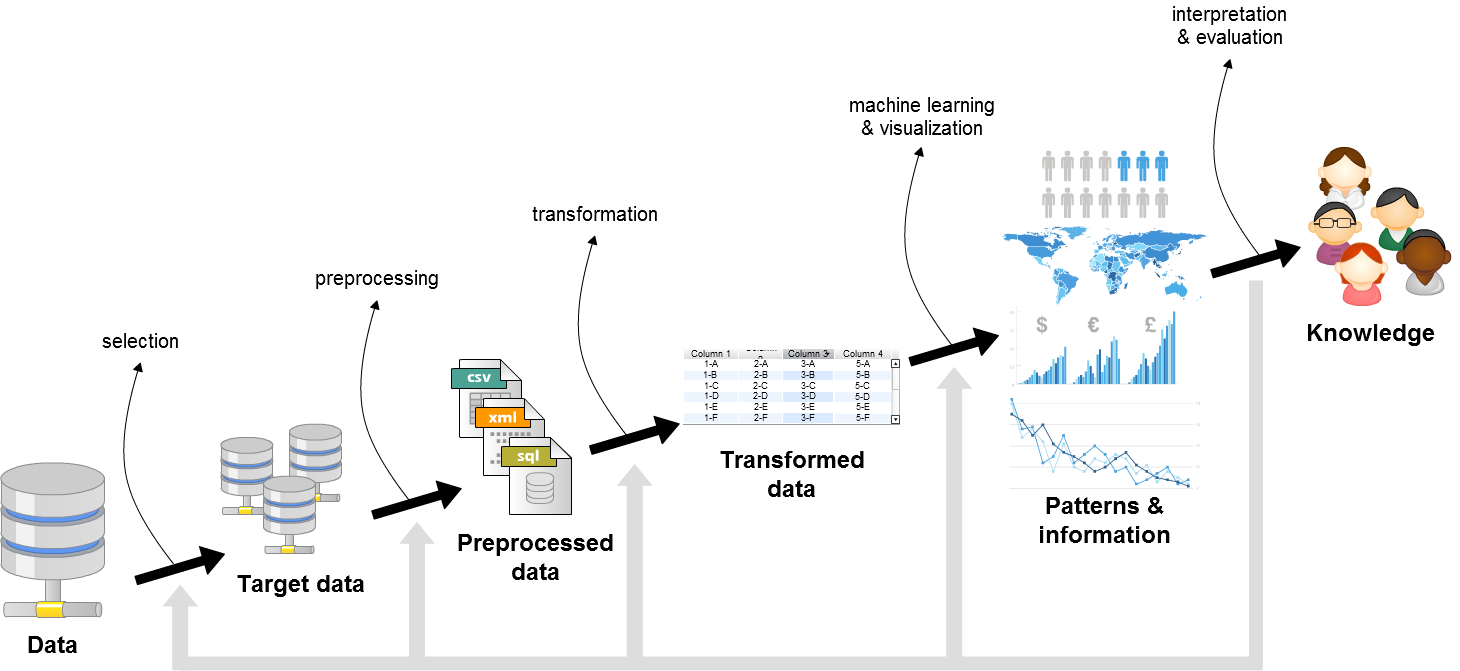
\includegraphics[width=0.9\linewidth]{figures/Untitled.png}
	\caption{Data mining as a process, from data acquisition to knowledge discovery. Source: adapted from \textit{From Data Mining to Knowledge Discovery in Databases}~\cite{Fayyad:1996:DMK:257938.257942}}
	\label{fig:data-mining}
\end{figure}

Data mining enables a better understanding of human or natural processes and provides us with means to identify trends, predict future events or discover useful patterns. Its uses range from scientific and medical applications to social sciences or business administration~\cite{Fayyad:1996:DMK:257938.257942}.

\subsubsection{Facing the limits}

Despite lots of effort is put into enhancing different data mining processes, there still are many cases where these techniques fail to perform correctly; mainly, it is a matter of scale.

On one hand, traditional data mining workflows cannot cope with the really massive data sets that are available nowadays, if performed on a common infrastructure. To solve this issue, clusters of hundreds or thousands of computers are used to run such analysis. It is costly and complex but, doing so, we can mine data that we couldn’t some time ago.

On the other hand, we face another type of scaling problem. In some situations, data acquisition throughput is so high that it can’t be stored anyway, so another approach is needed to avoid the loss of information that it could deliver us. Moreover, we might not want to store it, even when we could, but yet we want to analyze it to extract knowledge from it, as soon as we received it. Both scenarios are addressed with a series of techniques known as \textit{stream mining}.

\subsubsection{Stream mining}

Stream mining or data stream mining is a process that allows us to still discover knowledge and patterns in data, even when it comes in the form of a continuous stream, or many of them~\cite{Rajaraman:2011:MMD:2124405}. Instead of processing all statically stored data, like traditional data mining does, a relatively small portion of it is kept during the analysis, and it is updated when needed - either because more resources are available to the system or because new data is acquired. A more deeper review of this research area is given in section~\ref{section:state-of-the-art}.

\textbf{Stream mining in this project:}

MOA, initials for Massive Online Analysis, is an open source framework for data stream mining~\cite{website:MOA-Overview}, originally developed at the University of Waikato, New Zealand. It includes several machine learning algorithms\footnote{Algorithms used to perform the actual data mining analysis (the “machine learning \& visualization” step on figure~\ref{fig:data-mining}) belong to the field of machine learning. In MOA, clustering, classification, regression, outlier detection and recommender systems are available.} to perform the analysis and tools to evaluate the quality of the results. It also deals with a problem known as \textit{concept drift}\footnote{It is said of statistical properties of a target variable being analyed, when they change over time in unforeseen ways.}. It is related to the Weka\footnote{Weka is a popular software package including classical data mining algorithms, this is, not stream mining. It is also developed at the University of Waikato.~\cite{website:Weka}} package, but it is built to perform at a greater scale for more demanding problems.

\subsection{Privacy}

Privacy is a concept that can be defined as the ability of an individual or group to seclude\footnote{“Seclusion is the act of placing or keeping someone away from other people.” Source: Merriam-Webster online dictionary~\cite{website:merriamSeclusion}} themselves, or information about themselves, and thereby express themselves selectively. It is understood differently depending on the social and cultural background of each individual, but it is in fact recognised as one of the most fundamental rights of our human nature. The Universal Declaration of Human Rights’ 12th article~\cite{website:humanRights} states that:

\begin{quote}
No one shall be subjected to arbitrary interference with his privacy, family, home or correspondence, nor to attacks upon his honour and reputation. Everyone has the right to the protection of the law against such interference or attacks.
\end{quote}

This right has been continuously violated ever since information exchange and advanced communication technologies have been developed. Despite this did not begin with the spread of the Internet, its adoption has greatly magnified both the ability to breach people’s privacy and the impact that these breaches have.

\subsubsection{Privacy leaks consequences}

We are fully aware of the dramatic consequences that information leaks have caused these past years; for example, the \textit{PlayStation Network} outage which left millions of video gamers without access to this service~\cite{playstation1} or the more recent celebrity intimate photographs leaks~\cite{celebrities}. Even though they are referred to as "IT security breaches" in the media, they are indeed privacy right violations, because sensitive personal information was compromised in both examples.

Economical and social consequences are at stake too: identity thefts are performed on a daily basis thanks to the vast amount of data about individuals available in the web. Back in 2005, the cost of these thefts was estimated to be in the order of billions of dollars~\cite{DisclosureLaws}.

\subsubsection{Legal framework}

Efforts are being carried out to develop legal frameworks to help protect people’s privacy, at many levels. One such example is the spanish LOPD\footnote{LOPD stands for \textit{Ley Orgánica de Protección de Datos}, a law that was approved by the spanish courts in 1999. It has been modified several times, being the law enforcement regulation approved in 2007.}~\cite{lopd}, a law that, among other things, defines different data privacy levels and, for each of them, mandatory proceedings, protocols and data protection methods.

There are some pitfalls to these legislative efforts, though. Firstly, it is really hard to assess their accomplishment in the IT sector and, thus, it is sometimes a matter of confidence in the developers good practices and ethic behaviours. Another important drawback is that online services, such as social networks, can be accessed globally, but, on the other hand, their legislative framework is that of the country to which the backing company offering the service belongs to - jurisdiction definition in the Internet is still a matter of intense debate, nowadays.

\subsubsection{Privacy and data mining}

Data mining technologies have also become a relevant debate topic nowadays, concerning what information is collected from individuals, who owns it and what are the purposes behind its gathering. Information technologies deliver us many benefits at many levels - safer streets, cheaper communications, better health systems, more convenient shopping - but at the high cost of losing our privacy.

Knowledge discovery processes need data to work and, in most cases, it is sensitive and personal. Moreover, it is massively collected and stored and analyzed without us knowing much about it. Besides the lack of consent in this data acquisition stage of the process, data mining poses a bigger thread on individuals: information disclosure. Sensitive data must be treated accordingly, which involves not only good IT security practices to avoid leaks like the ones described before, but a responsible treatment when research results are published.

Statistical Disclosure Control (SDC) is the name that the statistical community has given to what the data mining community calls Privacy-Preserving Data Mining (PPDM). This field, whatever its preferred name is, deals with controlling that information about specific individuals is not extracted from statistical summary results. Also, if full datasets are to be released, PPDM methods should be applied to data in order to preserve user's privacy, whilst maintaining the statistical significance of it, i. e., the amount of information - knowledge - that this data can provide.

Further details of SDC methods and approaches can be found in the State of the Art section~(section~\ref{section:state-of-the-art}).

\subsection{Involved stakeholders}

To further understand the motivation driving this project we can examine which third parties are involved in it, giving a general overview of their possible interests in this work.

\subsubsection{Users: organizations and developers}

The most direct users of the results of this project will be developers, data scientists\footnote{The term \textit{data scientist} is used to designate the evolution of data analysts or business analysts job titles in the world of \textit{Big Data} or data mining. They are trained in computer science and its applications, modeling, statistics, analytics and mathematics.}, researchers and the companies and organizations that employ them. Using privacy preserving filters they are allowed to release their results or data sets without compromising their users privacy. National statistical agencies\footnote{The ONS (Office for National Statistics, in the UK) team is using statistical disclosure control methods as part of their process methodology~\cite{website:sdc}.} and private enterprises might find it useful as well.

\subsubsection{End users: data providers}

Data providers (anyone that allows collection of their data) get the most important benefit from privacy preserving data mining: their data is secure against information disclosure attacks. Because all kinds of sensitive data is kept and analyzed, this happens to be the main motivation for the project - even though data providers might not be aware of the specific technologies that keep their data safe, they still have the right to demand this protection.

\subsection{State of the art}
\label{section:state-of-the-art}

\subsubsection{Stream mining}

Data stream mining is a relatively new field. Even though its theoretical foundation is based in well-established statistical and computational approaches, it has not been until recent years that this research area has experimented such growing interest.

The main problem when dealing with streaming data is the high throughput of data being analyzed, under computational resources constraints. Variable data rates is another problem that has to be addressed too. Once these problems are resolved, efforts are done so the same kind of data mining analysis as in the case of batch data processing are available: classification, regression or clustering tasks, as well as outlier detection and recommendation systems. We will not cover these techniques here, because they are not related to this project, by themselves. Instead, we will have a look at some different stream mining solutions, because their working principles do affect the way the project’s algorithms will be implemented.

Solutions provided in this field can be categorized into \textit{data-based} and \textit{task-based} ones~\cite{miningDataStreams}, depending on their approach.

\begin{itemize}
	\item \textbf{Data-based stream mining solutions:}
	The idea behind these solutions is to use a subset of the original dataset to perform the required analyses. Diverse techniques that have been used in this sense can further be split into two more categories:
	\begin{itemize}
		 \item \textit{Sampling methods:} either by randomly picking samples of the data stream or by randomly selecting chunks (subsets) of the stream, sampling methods discard part of the incoming data, while performing the knowledge discovery processes with the sampled data. The main problem with this approach is that is hard to know when to pick a sample or which records should be stored, because there is no previous knowledge of the dataset size or its information structure.
		 
		 \item \textit{Summarizing methods:} they use aggregated data or calculated statistical measures (that are continuously recalculated) to provide the information needed for the data mining algorithms. In this case, it is the loss of information and accuracy and the inability to control data distribution fluctuations what renders these methods not so usable as it was desired.
	\end{itemize}
	
	\item \textbf{Task-based stream mining solutions:}
	The solutions that fall into this category are based not on performing data transformations, but on changing the data mining methods to enable their use on data streams.
	\begin{itemize}
		\item \textit{Approximation algorithms:} these are a kind of algorithms that are designed to solve computationally hard problems, by giving an approximate result. Instead of computing exact solutions, they just guarantee a certain error bound. The problem with these methods is, again, the high received data throughput, which they cannot cope as well. Additional tooling is therefore needed if one wishes to use them.
		
		\item \textit{Sliding window method:} this method, a common pattern in many online\footnote{In computer science, an \textit{online algorithm} is one that can process its input piece-by-piece in a serial fashion, i.e., in the order that the input is fed to the algorithm, without having the entire input available from the start.} applications, maintains a \textit{sliding window} in which the most recent data is kept. As data is received from the incoming streams, this window “advances” so new observations are kept inside. The data mining analyses are then performed using the data available inside the window and summarized versions of the older records, in the form of statistical measures or aggregated data.
		This particular method is the one that the MOA package uses - thus its name: Massive \textbf{Online} Analysis. This solution scheme enables dealing with concept drift, which would not be possible if just aggregated data was used.
		
		\item \textit{Algorithm output granularity:} this method is a resource-aware data analysis approach that can perform the local analysis on resource constrained devices, by adapting to resource availability and data stream rates - when resources are completely running out, the results are merged and stored.
	\end{itemize}
\end{itemize}

\textbf{Data stream mining software:} because it is an incipient field, stream mining software packages are quite uncommon. Even though specific applications have been developed~\cite{mineFleet}, MOA remains as one of the few generic\footnote{MOA is not focused towards any particular application scenario: it is a base tool with which we can build such specific systems.}, free and open sourced systems.
In relation to MOA, a new project called SAMOA~\cite{samoa} is being developed too, based on top of MOA itself, and a couple of streaming processing engines: Apache S4~\cite{apacheS4} and Apache Storm~\cite{apacheStorm}, developed by the Apache Software Foundation.

\subsubsection{Privacy preserving stream mining}

Many different methods have been developed to help prevent information disclosure when data mining datasets or results are released. These algorithms pursue the generation of results or data that have particular properties concerning privacy preservation.

\textbf{Privacy preserved data properties:} some of the desirable properties of privacy-protected data are:
\begin{itemize}
	\item First described in 2002, by Latanya Sweeney, a release of data is said to have the \textit{$k$-anonymity} property if the information for each person contained in the release cannot be distinguished from at least $k-1$ individuals whose information also appears in the release~\cite{kAnon}.
	
	\item The evolution of the concept of $k$-anonymity is \textit{$l$-diversity} and adds further privacy preservation by adding intra-group diversity, so to avoid the flaws of the $k$-anonymity privacy model~\cite{lDiversity}.
	
	\item Further on, the \textit{$t$-closeness} property definition adds attribute-based privacy enforcement to the $l$-diversity model: to better preserve privacy, all values (all observations) from a particular attribute must not be too much different - instead, they should be close up to a certain threshold~\cite{tCloseness}. This is needed to preserve the privacy of those records that are more easily identifiable because their attribute values are more distinguishable.
\end{itemize}

\textbf{Privacy preserving algorithms:} the algorithms being used nowadays to achieve effective privacy preserving properties to datasets can be categorized into the following groups~\cite{book:StatisticalDisclosureControl}:
\begin{itemize}
	\item \textit{Non-perturbative data masking:} these kind of methods do not perform data values transformations. Instead, they are based in partial suppressions of records or reductions of detail of the datasets. Some examples\footnote{We can’t cover every algorithm in detail, because some of them are not relevant and because those which are to be implemented in this project will be described in detail in the final project report.} are:
	\begin{itemize}
		\item Sampling
		\item Global recoding
		\item Top and bottom coding
		\item Local suppression
	\end{itemize}
	
	\item \textit{Perturbative data masking:} these methods do release the whole dataset, if required, but it is perturbed, this is, values are changed by adding them noise. This way, records are diffused and reidentifying individuals is harder. Some examples are:
	\begin{itemize}
		\item Noise masking
		\item Micro-aggregation
		\item Rank swapping
		\item Data shuffling
		\item Rounding
		\item Re-sampling
		\item PRAM
		\item MASSC
	\end{itemize}
\end{itemize}

\textbf{Privacy preserving \textit{Stream} Mining:} many of the previously listed methods are already implemented in many classical data mining frameworks and software systems; for example, the \texttt{sdcMicro} package for the \textbf{R} statistical package~\cite{sdcMicro}. However, privacy preserving methods are still not widespread in the stream mining ecosystem - that is another motivation for this project.

\subsection{Environmental impact}

No relevant direct environmental impact is related to this project, neither tied to its development nor its further deployment. No use of massive resources is done and the results of the work will not, presumably, result in a significant environmental change of any kind.

It is still true, however, that data mining, as a discipline and its broad use, does consume a lot of resources, in terms of technological infrastructure and energy. We cannot forget that collecting, storing and processing data at the industry scale needs entire data centers fully dedicated to the data mining process. Power consumption is a big concern with nowadays information technology, as it is the huge amount of rare materials that electronic devices contain. These are derived or indirect effects of the data mining process. This issue deserves to be examined more closely, in the project’s final report.

\subsection{Social impact}

Concerning social impact, this project’s strength is related to users privacy preservation through the implementation of algorithms that help anonymize their data within the data mining process. This topic will be explained more extensively in the project’s final report, but it is of paramount importance nowadays. Privacy is being relegated to the background with the advent of new information technologies, devices or platforms such as social networks or banking applications. Data is gathered from everyone and there is an increasing need of methods to protect it. Together with other fields more focused in securing the access to data, privacy-preserving data mining is designed to keep data safe at the analysis stage of the data mining process.

Not only ethical concerns are addressed by protecting the users’ privacy, but economical issues too. Industrial-scale information theft has a huge impact on enterprise economies, because of distrust and because disclosed sensitive data can be used to make profit of it.
